\chapter{Organisme d’accueil et problématique traitée}

\section{Introduction}
Le but de ce chapitre introductif est de mettre le travail dans son contexte général. Nous commençons tout d’abord par une présentation de l’entreprise d’accueil Sofia Technologies. Ensuite,nous réservons la deuxième partie pour détailler le cadre du projet et la méthodologie de travail adoptée.
%. Nous clôturons par lister les objectifs à atteindre,le langage et la méthodologie de conception à adopter.
\section{Organisme d'accueil}
Notre stage d’été a été effectué au sein de l’entreprise « SOFIA Technologies », une société de service {\@ IT} spécialisée dans le développement des solutions Cloud et Internet des objets fondée en 2011.\\
Les services développés par SOFIA Technologies sont: 
\begin{itemize}
\item Proposition des technologies logicielles avancées, de classe mondiale, conçues pour répondre aux besoins des entreprises.
\item  Une expertise dans toute la chaine de valeur de l’IoT: hardware, software et Big Data.
\item Une migration des infrastructures informatiques actuelles vers le cloud.
\item Le consulting.
\end{itemize}

% On peut ajouter une figure en utilisant le syntaxe suivant:
%\begin{figure}[htpb]
%\centering
%\frame{\includegraphics[width=0.5\columnwidth]{Logo_Entreprise}}
%\caption{Logo Entreprise}
%\label{fig:logo_tt}
%\end{figure}
\section{Problématique traitée et travail demandé}
Les formulaires présentent un outil indispensable dans la gestion des différentes ressources dans une entreprise.Mais, bien qu'il existe tant de générateurs de formulaires en ligne, chacun réponde à des besoins différents.
C'est pour cela, Sofia technologies a proposé la conception et le développement d'un POC de générateur de formulaire propre à elle afin d'améliorer la qualité de ses services.
\section{Choix méthodologique}
Dans cette section nous allons présenter le choix de la méthodologie et du langage adoptés dans la réalisation de notre projet.
\newpage
\subsection{Langage de modélisation}
Pour modéliser les fonctionnalités que doit offrir notre système, nous avons choisi le langage de modélisation UML puisqu'il s’agit d’un langage simple, formel et basé sur les notions de l’orienté objet.
\subsection{Méthodologie de conception}
La méthodologie est un procédé adopté afin de nous formaliser les étapes à suivre pour le développement du projet et pour que ce dernier répond rapidement aux besoins du client et réduit le  temps de production tout en minimisant les risques.\\
Dans cette optique, nous avons opté pour la méthodologie Agile Scrum au cours de notre projet.
La méthodologie Scrum valorise la notion de partage et d’équipe, elle implique l’intervention de trois rôles principaux qui sont spécifiés dans notre projet de la façon suivante :\\
- \textbf {Le Scrum Master }: son rôle est d'aider l'équipe à avancer dans le travail de manière autonome en cherchant en permanence à s’améliorer. Il surveille le bon déroulement du
projet et fournit un bilan à la fin de chaque sprint.\\
- \textbf {Product Owner }: La création du Product Backlog, une liste ordonnée de tout ce qui pourrait être requis dans le produit et son maintien sont les activités principales du Product Owner.\\ 
- \textbf {Équipe de développement }: Cette équipe assure qu'à la fin de chaque Sprint un incrément terminé soit livrable.
\section{Chronogramme des tâches menées durant le stage}
Au cours de cette section, nous allons déterminer les tâches de notre projet. Puis, nous
allons les ordonnancer dans le temps dont le but de faire une estimation de la durée occupée
par chacune d’elles et de suivre l’avancement du projet.
Pour cela nous avons modélisé la planification de notre projet en utilisant le diagramme de GANTT.\\
La figure \ref{figger} illustre le diagramme de Gantt de notre projet.
    \begin{figure} [H]
    \centering
         \begin{center}
             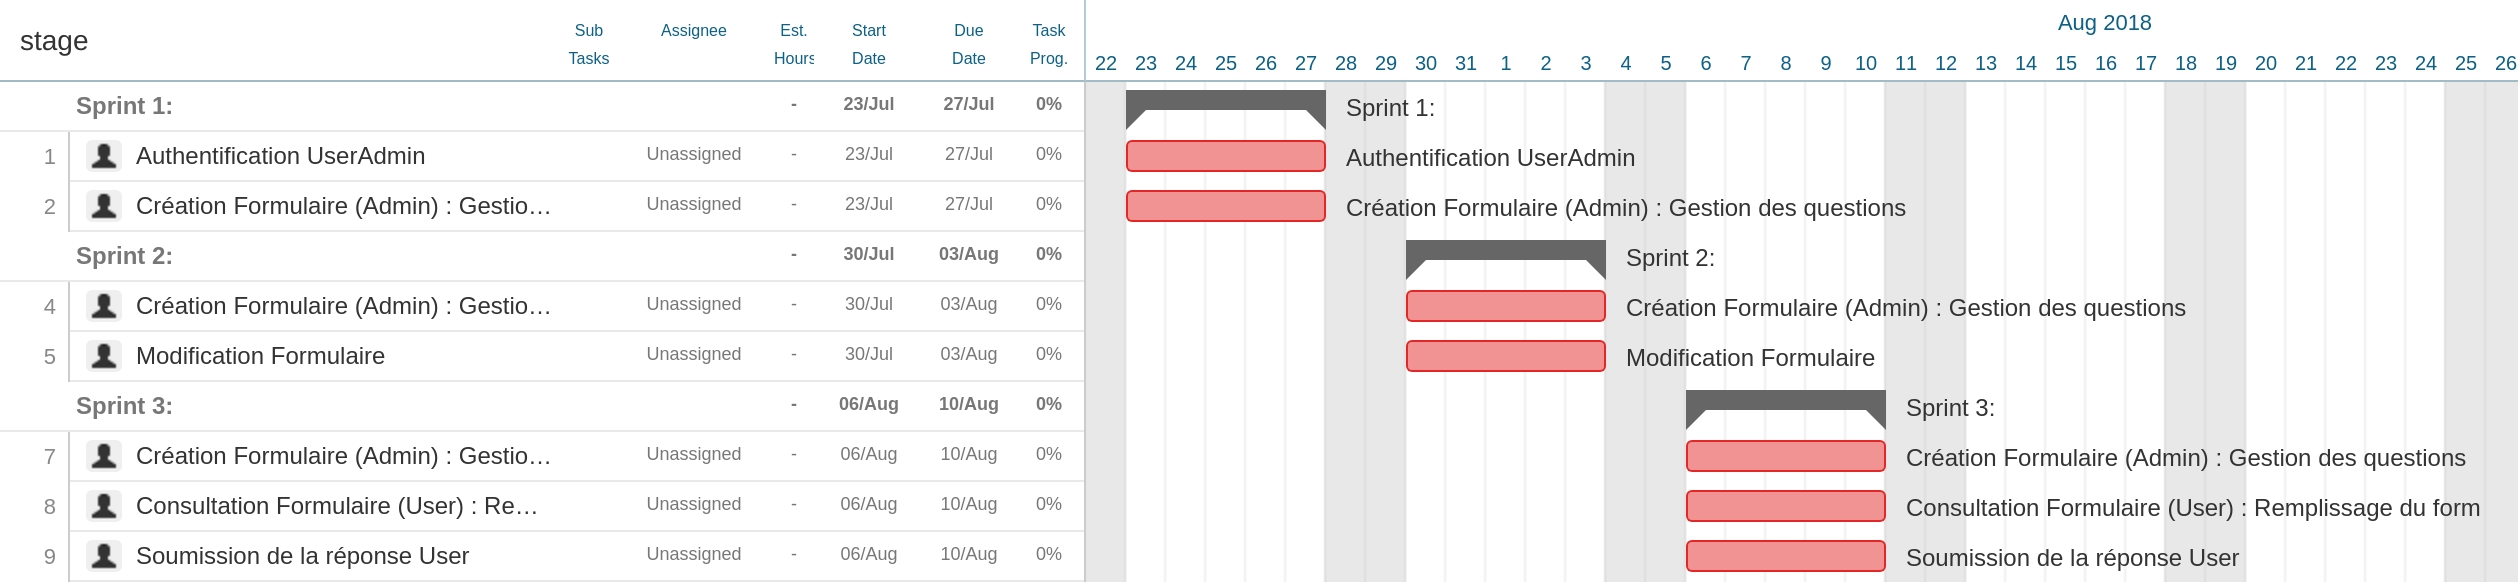
\includegraphics [width=18cm,height=9cm] {img/GANTTdiag.jpg}
            \caption{Diagramme de GANTT}
            \label{figger}
        \end{center}
    \end{figure}
    
\section{Conclusion}
Tout au long de ce chapitre, nous avons pu situer le cadre général de notre stage, à savoir la présentation du travail et ses objectifs, la société d’accueil et le cahier des charges proposé. Nous avons étayé aussi le choix du langage et la méthode de travail à utiliser.
Ce premier chapitre nous a introduit le contexte général du sujet à réaliser, le chapitre suivant sera entièrement consacré pour une étude conceptuelle du projet y compris l'analyse et l'étude des besoins du projet et son conception.